% ------------------------------------------------------------------------
%	Latex Preamble:  Formatting and Custom Commands
% ------------------------------------------------------------------------
\documentclass[12pt]{article}

\usepackage{amsmath, graphicx, subfig}

% to control the page number location and running title
\usepackage{fancyhdr}

% For the draft
\usepackage{endfloat}

% To control the spacing
\usepackage{setspace}

% For including code1
%\usepackage{listings}

% For using s
\usepackage{url}

% Citations are numbers, with round parenthesis
% no brackets around numbers in the bibliography
% use the CBE/CSE bib style
\usepackage[numbers,round]{natbib}
\renewcommand{\bibnumfmt}[1]{#1.}
\bibliographystyle{mrm}

% Equations have square brackets around them
\makeatletter
  \def\tagform@#1{\maketag@@@{[#1]\@@italiccorr}}
\makeatother

% Spacing and indentation
\topmargin -0.4in
\headheight 0.45in
\oddsidemargin 0in
\evensidemargin 0in
\textwidth 6.5in
\textheight 9in

\setlength{\parindent}{0pt} % No paragraph indent.
\setlength{\parsep}{12pt}   % Paragraph separation.
\setlength{\parskip}{12pt}  % Paragraph skip.

% Set the graphics path
\graphicspath{{./figures/}}


% ------------------------------------------------------------------------
%	Document start
% ------------------------------------------------------------------------
\begin{document}

\lhead{ISMRM Raw Data Format}
\chead{}
\rhead{\thepage}
\lfoot{}
\cfoot{}
\rfoot{}

% ------------------------------------------------------------------------
%	Full Title Page
% ------------------------------------------------------------------------
\newpage
\clearpage
\pagestyle{empty}

\begin{center}
\large \textbf{ISMRM Raw Data Format: A Proposed Standard for MRI Raw Datasets}

\normalsize
\singlespacing
Souheil J. Inati$^1$,
Joseph D. Naegele$^1$, 
Nicholas R. Zwart$^2$,
Vinai Roopchansingh$^1$,
Martin J. Lizak$^3$,
David C. Hansen$^4$,
Chia-Ying Liu$^5$,
David Atkinson$^6$,
Peter Kellman$^7$,
Sebastian Kozerke$^9$,
Hui Xue$^7$,
Thomas S. S{\o}rensen$^8$,
Michael S. Hansen$^7$
\end{center}

\begin{enumerate}
\item National Institute of Mental Health, National Institutes of Health, Bethesda, MD
\item Keller Center for Imaging Innovation, Barrow Neurological Institute, Phoenix, AZ
\item National Institute of Neurologic Disease and Stroke, National Institutes of Health, Bethesda, MD
\item Department of Oncology, Aarhus University Hospital, Aarhus, Denmark
\item Radiology and Imaging Sciences, Clinical Center, National Institutes of Health, Bethesda, MD
\item Centre for Medical Image Computing, University College London, United Kingdom
\item National Heart, Lung, and Blood Institute, National Institutes of Health, Bethesda, MD
\item Department of Clinical Medicine, Aarhus University, Aarhus, Denmark
\item Institute for Biomedical Engineering, University and ETH Zurich, Zurich, Switzerland
\end{enumerate}

\vspace{2mm}
Correspondence to: \\
Souheil J. Inati \\
National Institue of Mental Health, NIH \\
NIH Building 10/1D-70 \\
10 Center Drive \\
Bethesda, MD 20892 \\
\textit{souheil.inati@nih.gov} \\

\textit{Running Head:  ISMRMRD}

\vspace{2mm}

\textit{Submitted to Magnetic Resonance in Medicine} 

\vspace{2mm}

\textit{Word count: 3904} % reported by texcount (total-abstract-top)


% ------------------------------------------------------------------------
%	Abstract
% ------------------------------------------------------------------------
\newpage
\clearpage
\pagenumbering{arabic} % begin numbering here
\pagestyle{fancy}
\doublespacing
\section*{Abstract}
\textbf{Purpose:}  This work proposes the ISMRM Raw Data (ISMRMRD) format as a common MR raw data format, which promotes algorithm and data sharing.\\
\textbf{Methods:} A file format consisting of a flexible header and tagged frames of k-space data was designed. Application Programming Interfaces were implemented in C/C++, MATLAB, and Python. Converters for Bruker, General Electric, Philips, and Siemens proprietary file formats were implemented in C++. Raw data were collected using MRI scanners from four vendors, converted to ISMRMRD format, and reconstructed using software implemented in three programming languages (C++, MATLAB, Python).\\
\textbf{Results:} Images were obtained by reconstructing the raw data from all vendors. The source code, raw data, and images comprising this work are shared online, serving as an example of an image reconstruction project following a paradigm of reproducible research.\\
\textbf{Conclusion:} The proposed raw data format solves a practical problem for the MRI community.  It may serve as a foundation for reproducible research and collaborations.  The ISMRMRD format is a completely open and community-driven format, and the scientific community is invited (including commercial vendors) to participate either as users or developers.

\textit{Abstract word count: 197} % reported by texcount (abstract)

% ------------------------------------------------------------------------
%	Keywords
% ------------------------------------------------------------------------
\textbf{Keywords:}  MRI, Image reconstruction, Open source, Raw data format

% ------------------------------------------------------------------------
%	Body
% ------------------------------------------------------------------------
\newpage
\clearpage
\onecolumn

% ------------------------------------------------------------------------
%	Introduction
% ------------------------------------------------------------------------
\section*{Introduction}
Image reconstruction research has played a pivotal role in driving many advances in magnetic resonance imaging. Examples of paradigm shifting techniques include parallel imaging~\cite{Pruessmann:1999uq, Sodickson:1997fk, Griswold:2002kx}  and, more recently, the introduction of nonlinear reconstruction and compressed sensing~\cite{Donoho:2006compressed, Lustig:2007vn}. Novel reconstruction algorithms build on and improve existing methodology, and most reconstruction articles compare new methods to existing methods in terms of image quality and reconstruction speed.

Reproducible research has drawn a great deal of attention recently, as highlighted for example in a recent special issue of Science~\cite{Jasny:2011again, Peng:2011reproducible}. The field of computational science in particular has produced several excellent examples of how such research can be carried out, e.g., the wavelab toolbox~\cite{wavelab}.  The ISMRM has begun to take steps to help facilitate reproducible research, e.g., with the MRI unbound website~\cite{mri_unbound}. Underlying many of these efforts is a discipline-specific file format specification that allows scientists to exchange data easily.  Much of modern astronomy research, for example, relies on telescope data in the FITS standard~\cite{fits}.  Other discipline-specific data formats have enabled scientists to escape from the limitations imposed by vendor-specific, proprietary technology, leading to the development of a wide range of post-acquisition data analysis tools, and enabling large-scale collaborations.  Medical imaging has the DICOM standard~\cite{dicom}, which allows radiology departments to store data from different vendors on a centralized PACS, and computer scientists to implement novel image processing methods in a vendor neutral manner. The subfield of neuroimaging has NIfTI~\cite{nifti}, which underlies large-scale projects like the human connectome project~\cite{connectome}. The image file formats are useful for disciplines that operate on the reconstructed images, but they do not address the needs of scientists involved in the development of image reconstruction algorithms. This paper proposes an MR-specific raw data format. 

This ISMRMRD standard was developed by a subcommittee of the ISMRM Sedona 2013 workshop.  It is designed to capture the details of the MRI experiment in a way that permits image reconstruction.  It is important to note that this goal is fundamentally different from that of proprietary vendor raw data file formats.  Generally, proprietary vendor raw file formats are intended to capture protocol parameters for a particular pulse sequence at the time of the scan.  The proprietary raw data file formats are intended to store the information needed to reproduce a particular experiment on a specific version of the scanner software and reconstruction framework.  The tight coupling between 1) the scanner console user interface, 2) the pulse sequence control parameters, and 3) the image reconstruction control parameters, make the vendor formats depend on a great deal of proprietary, vendor-specific knowledge. The quantity of hidden information makes these formats inconvenient for data sharing.  More importantly, the specific implementation details of a particular vendor's scanner software architecture greatly influences the design of these file formats and the type of information that they contain.  In contrast, the proposed standard is designed to facilitate the exchange of the raw k-space data along with the physics parameters of the data acquisition process to provide the information necessary for image reconstruction.

While the ISMRMRD format will continue to evolve as it attracts more users with a more diverse set of applications and needs, the basic format has remained stable for more than two years, and it makes sense to present it to the MRI community. This paper lays out the design and structure of the format and describes several software tools that have been developed to interact with data in the proposed format. A number of vendor-specific tools have been created for converting proprietary data formats to the proposed format. An overview of the current status of these data converters and information needed to locate them is also provided. As a demonstration of how the data format can be used, a phantom has been scanned on four different scanners, the data converted to ISMRMRD and reconstructed with several different open source reconstruction programs written in Matlab (The MathWorks), Python, and C++ programming languages. 

All software, data, figures, scripts to generate the figures, and the text in this manuscript are available as open source. 


% ------------------------------------------------------------------------
%	Methods
% ------------------------------------------------------------------------
\section*{Architecture and Implementation}
\subsection*{Design}
The proposed ISMRMRD format combines a flexible header (XML-based) with fixed structures for the data. These are packaged together into a single file.  A minimal raw data set is depicted in Fig.~\ref{fig:format} and consists of two sections:
\begin{itemize}
\item{XML header.} A flexible XML format document that can contain an arbitrary number of fields and accommodate everything from simple values (matrix sizes, etc.) to entire vendor protocols, etc. The purpose of this XML document is to provide parameters that may be meaningful for some experiments but not for others. This XML format is defined by an XML Schema Definition file (\texttt{ismrmrd.xsd}).
\item{Raw data.} This section contains all the acquired data in the experiment organized as a sequence of data items.  Each data item corresponds to a single data frame or chunk in an experiment, for example, a single line of data in a Cartesian acquisition or a single interleave in a multi-shot spiral acquisition. Each data item consists of a fixed-size header (C-struct) with encoding numbers, etc., along with the k-space data for all of the acquired channels, and (optionally) the k-space trajectory as depicted in Fig.~\ref{fig:cstruct}. The raw data structures are defined in a C/C++ header file (\texttt{ismrmrd.h}).
\end{itemize}
The proposed format also provides a simple image format for storing the product of reconstructions and a multidimensional array format for storing additional user-specified parameters (e.g., gradient nonlinearity correction maps, etc.).

% Figure 1
\begin{figure}
\begin{center}
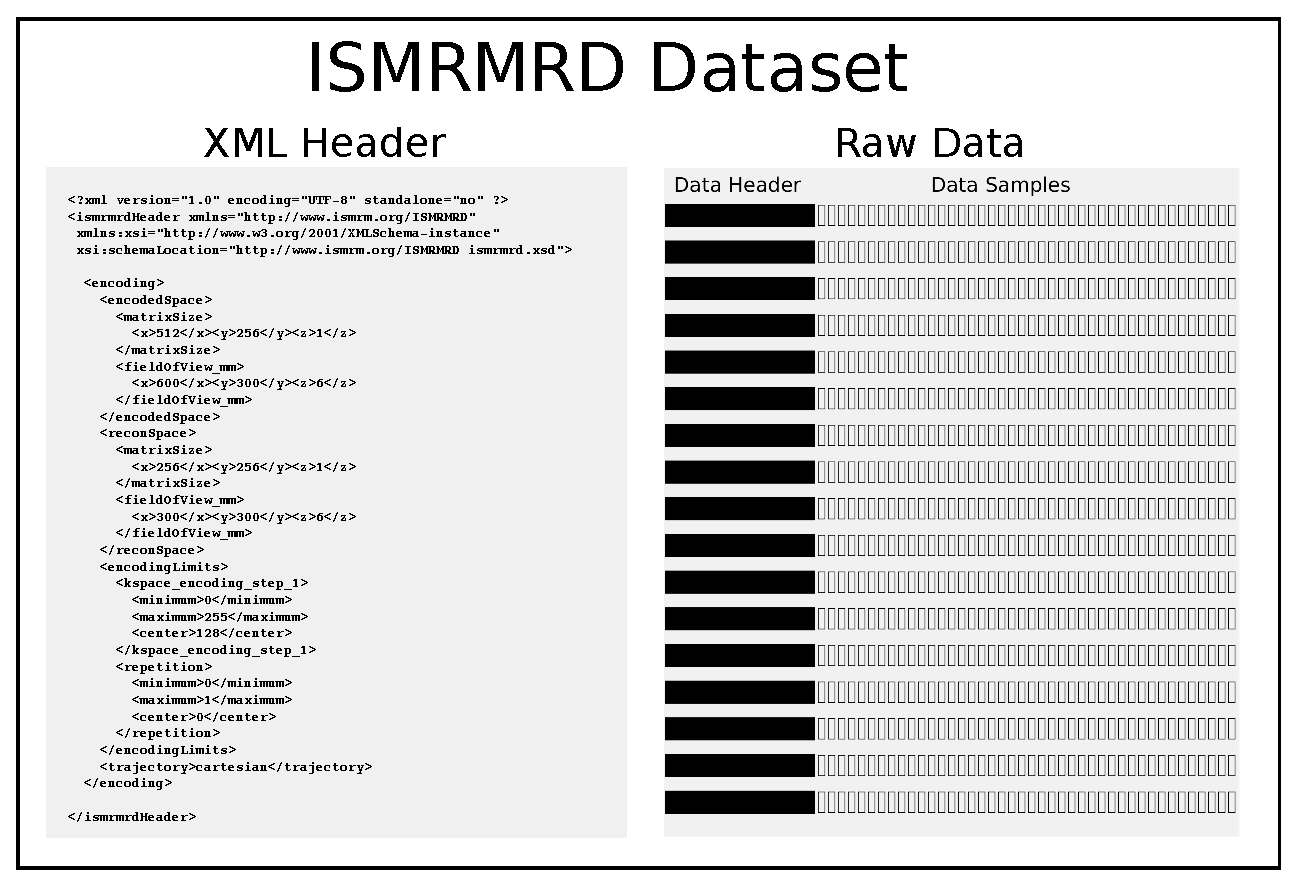
\includegraphics[width=6in]{figure1_ismrmrd_format.eps}
\caption{A minimal ISMRMRD dataset consists of a flexible XML header and raw data organized as sequence of data items consisting of fixed-size data headers and the corresponding k-space data for each set of samples or data chunk.}
\label{fig:format}
\end{center}
\end{figure}

% Figure 2
\begin{figure}
\begin{center}
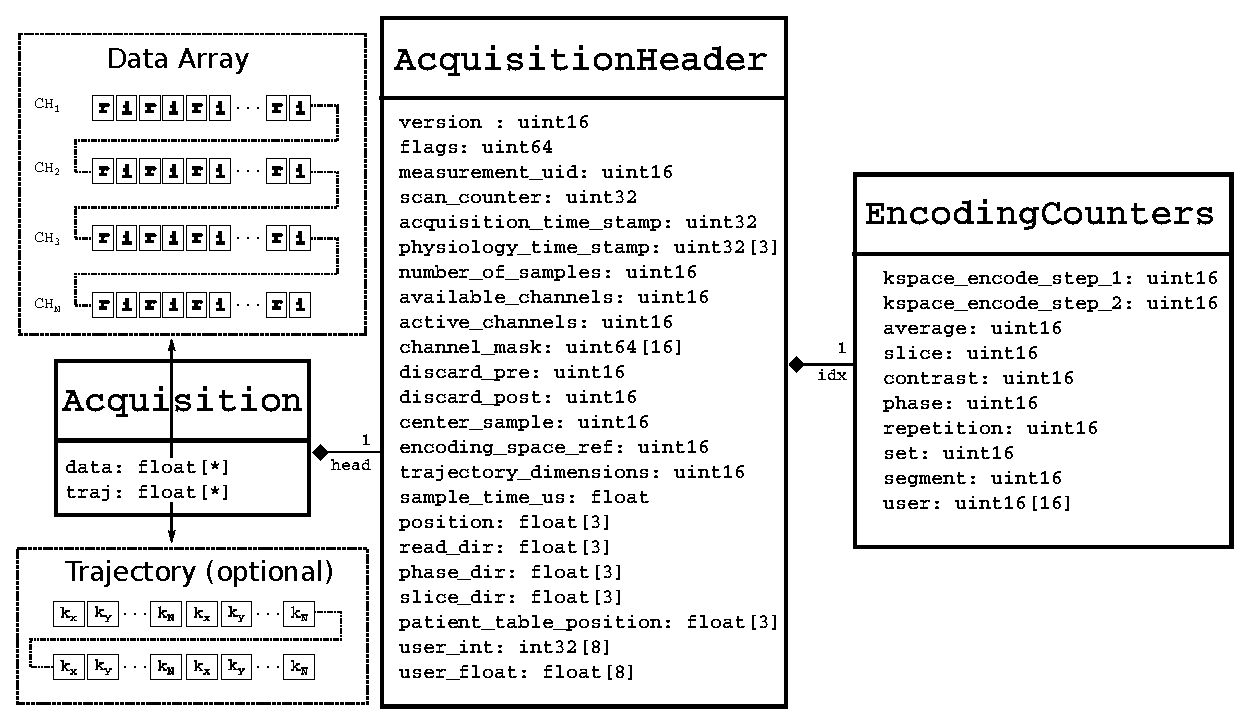
\includegraphics[width=6in]{figure2_uml_diagram.eps}
\caption{The raw data structure for each data frame or chunk of the acquisition, consisting of a fixed-size header with encoding numbers, location, etc. and the raw k-space data and (optionally) the k-space sampling locations. \textbf{r} and \textbf{i} indicate the real and imaginary part of the data points respectively.}
\label{fig:cstruct}
\end{center}
\end{figure}

One of the key design features of the proposed format is the notion of an ``encoding space", which is a description of the type and limits of the experiment and provides the reconstruction program with the physical size and resolution of the imaging volume and the ranges of the data header labels.  An ISMRMRD dataset may contain data from several encoding spaces.  Each encoding space is described in the XML header, and each acquisition (data chunk) is tagged with a label for the encoding space from which it was acquired. All encoding spaces have a trajectory type, an ``encodedSpace," a ``reconSpace", ``encodingLimits", and an optional trajectory description, that can contain an arbitrary set of named parameters such as the gradient ramp and flat top times for EPI, or the parameters controlling the shape of the spiral trajectory, etc.  An example of an encoding describing a simple 2D Cartesian acquisition is shown in Fig.~\ref{fig:encoding}.  In this particular case, the encoding has the following description:
\begin{itemize}
\item the ``encodedSpace" section gives the matrix size ($32\times16\times1$) and field of view in mm ($600\times300\times10$) of the imaging volume encoded by the excitation, i.e.,  a 10~mm thick slice, 600~mm in x and 300~mm in y, encoded with a nominal matrix size of 32 in x and 16 in y, i.e., at a nominal resolution of 18.75mm.
\item The ``reconSpace" section indicates that the image should be reconstructed on a smaller field of view ($300\times300\times10$), but with half the number of pixels in x.
\item The combination of the ``encodedSpace" and ``reconSpace" indicates that the k-space data were acquired on a grid oversampled by a factor of 2 in the x direction.
\item The ``encodingLimits" section indicates the ky center (5) and the minimum and maximum ky values (0 and 11 respectively), i.e., this is a partial Fourier experiment, with a true pixel size that is somewhat larger than the nominal resolution, $min(ky)=-5$, $max(ky)=+6$.
\end{itemize}
% Figure 3
\begin{figure}
\begin{center}
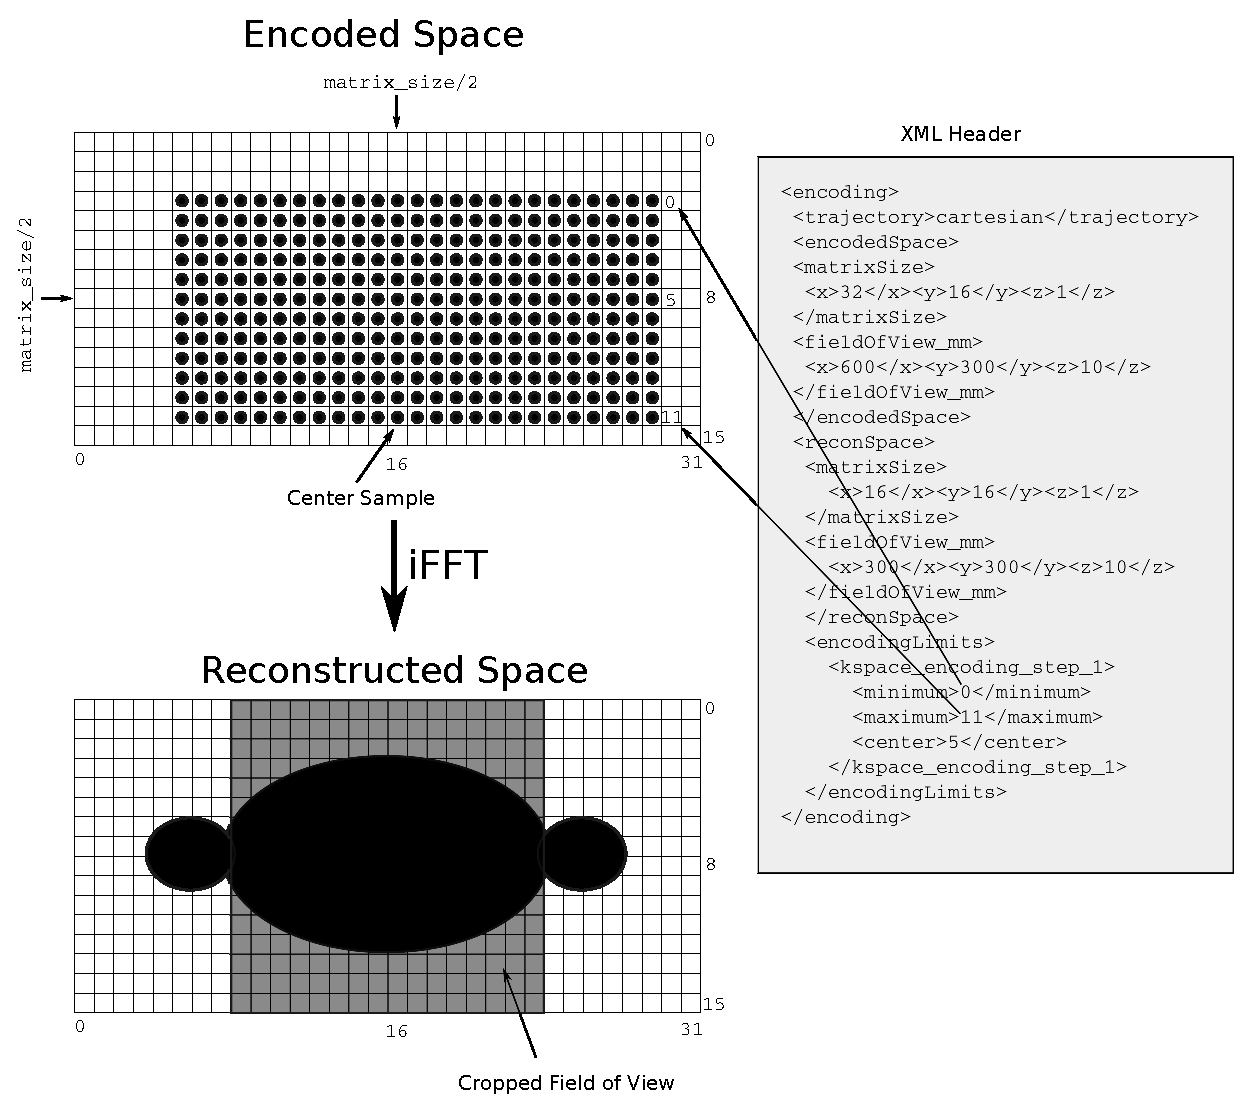
\includegraphics[width=6in]{figure3_encoding_spaces.eps}
\caption{The encoding space of a simple 2D Cartesian acquisition.  The XML header describes the image encoding and reconstruction fields of view and matrix sizes and k-space sampling bounding box.  The image is acquired at a matrix size of 32 $\times$ 16 $\times$ 1 and field of view of 600mm $\times$ 300mm with a slice thickness of 10mm.  It should be reconstructed at a matrix size of 16 $\times$ 16 $\times$ 1 and field of view of 300mm $\times$ 300mm with a slice thickness of 10mm.   The k-space data were acquired on a grid oversampled by a factor of 2 in the x direction.  The ``encodingLimits" section indicates the ky center (5) and the minimum and maximum ky values (0 and 11 respectively), i.e. this is a partial Fourier experiment, with a true pixel size that is somewhat larger than the nominal resolution, $min(ky)=-5$, $max(ky)=+6$. The example experiment also employs partial Fourier along the readout dimension, i.e. asymmetric echo.}
\label{fig:encoding}
\end{center}
\end{figure}


\subsection*{ISMRMRD Library}
The ISMRMRD library is a cross-platform implementation based on the Hierarchical Data Format (HDF) (\url{http://www.hdfgroup.org/HDF5}) for storage and provides C/C++, Python, and MATLAB (Mathworks) interfaces for reading and writing ISMRMRD files.  The project follows an open source development model with a website at (\url{http://ismrmrd.github.io}) and a discussion board and code repositories at \url{http://github.com/ismrmrd}.  The library and associated tools can be compiled in a straightforward way on Linux, Windows, and Apple computers.  This section provides a high-level description of the implementation and discuss some of the choices made during the development process.  The reader is encouraged to examine and experiment with the source code for more a detailed view.

\subsubsection*{File container}
The HDF format was chosen as the binary file container.  The HDF format is very flexible and has been adopted broadly in the scientific community.  Reading and writing from the HDF format are supported by most programming languages and computational environments.  The HDF library has a core C and C++ API, is supported natively in MATLAB (it forms the basis for MATLAB's own ``.mat" file format), and is supported in Python via the H5Py package (\url{http://www.h5py.org}).

\subsubsection*{XML header data binding}
The XML header can be thought of as a text representation of relevant experimental parameters that are needed for meaningful image reconstruction. When writing image reconstruction software, the software developer usually interacts with a binary representation of the XML document (XML Data Binding) to avoid direct, error prone, and tedious interaction with the XML text. The process of generating the binary representation of the XML document (deserialization) and the generation of the XML document from the binary representation (serialization) is handled by dedicated functions. Both the binary representation and the functions for serialization and deserialization can be auto-generated by XML data binding tools, e.g., CodeSynthesis XSD (\url{http://www.codesynthesis.com/products/xsd/}) for C++, JAXB for Java (\url{https://jaxb.java.net/}), or PyXB (\url{http://pyxb.sourceforge.net/}) for Python. The auto-generated data structures and functions are easier to maintain since they can be regenerated when the XML schema (\texttt{ismrmrd.xsd}) changes, but the syntax they provide can be less convenient. Alternatively, data structures and serialization and deserialization code can be "handcrafted". This may provide a more convenient interface, but the software maintenance overhead is greater. The proposed data format does not dictate which approach to use when interacting with the XML header, but the provided libraries include data structures and associated functions. Depending on the convenience of available tools these software components have either been "handcrafted" or auto-generated as described below.  

\subsubsection*{Programming language-specific implementations}
This work is implemented in three different programming environments or languages to interact with ISMRMRD files. This section contains a few notes regarding the C/C++, MATLAB, and Python APIs that were created:
\begin{itemize}
\item{C library.}  This code defines fixed data structures (\texttt{ismrmrd.h}) and the functions used to interact with the HDF5 file.
\item{C++ library.} This code is a wrapper around the C library with classes and functions that provide memory management and reduce programming error.  It includes a ``handcrafted'' XML header binding class.  
\item{Build system.} The C and C++ implementation use the CMake (Kitware) build configuration system to support multiple operating systems (Linux, Microsoft Windows, Apple OS X).
\item{MATLAB library.} This code consists of pure MATLAB data structures and functions (classes) that call the MATLAB interface to HDF5 as well as ``handcrafted'' Java code for the XML header binding class using the Java provided by MATLAB.
\item{Python library.} This code consists of pure Python classes for the data structures, uses NumPy arrays for the data and the k-space trajectories (\url{http://www.numpy.org}), and an auto-generated XML header binding class.
\end{itemize}

The code repositories also contain the source code for the documentation (which use the Doxygen (\url{http://www.doxygen.org}) and Sphinx (\url{http://sphinx-doc.org}) projects) as well as examples of how to use the APIs to read and write ISMRMRD files.

\subsection*{Data Conversion Tools}
Converters have been developed for several proprietary file formats: Bruker, General Electric, Philips, and Siemens.  The Bruker, Philips and Siemens converters are open source with repositories that can also be found at \url{http://github.com/ismrmrd}.  The GE converter relies on proprietary vendor code and is being distributed via the vendor's research network.  Given the variety in vendor raw data file formats, the architecture of these programs is described in general terms with the aim of giving some guidance or aid to others who are implementing their own conversion tools.  The reader is referred to the source code for  details, but to give a few examples: the Bruker raw data are stored in a simple directory structure with the acquisition parameters stored in several text files and k-space data stored in a simple binary file as equal length frames of k-space data; there are no data labels associated with each data frame. Siemens raw data are stored in a single integrated file that can contain raw data from multiple scans.  For each scan, acquisition parameters are stored in a structured text header, followed by k-space data frames stored in acquisition order, where each frame of k-space data is tagged with data labels containing the frame's line number, slice number, location, etc. The complexity of the GE and Philips formats fall somewhere between the simple file structure of the Bruker format and the more integrated file format used on the Siemens systems. The GE data does not contain explicit labels for each data frame and more sequence knowledge is needed to convert the data. The Philips raw data format has data labels associated with each data frame and it was possible to design a more generic automated converter.   

The converters for the aforementioned vendor formats were written in C++. Acquisition parameters from the vendor-specific data were converted to an intermediate XML file (containing vendor-specific parameter names and values). This  XML file was then translated into the vendor-independent ISMRMRD XML header file using a sequence-specific Extensible Stylesheet Language (XSL) style sheet. The frames of k-space data were processed in the order in which they appeared on disk.  For formats with tagged data frames (Philips and Siemens), the proprietary binary header tags were parsed and used to populate the fixed-size ISMRMRD data header structures.  For formats with untagged data frames (Bruker and GE), sequence and vendor-specific knowledge was used.  

It is worth emphasizing that creating the converters required significant work and special knowledge of the vendor formats. However, once code was developed for converting raw data from one pulse sequence on a particular platform, it was straightforward to modify this code to handle other sequences. It is expected that other developers can modify these converters to handle currently unsupported product sequences or their own research sequences. It is also important to note that while some users may work on the implementation of these vendor-specific converters, many users will simply use the converted ISMRMRD files as input for the algorithms and thus be exposed less to these vendor-specific details as a consequence of using the proposed format. 

\section*{Experimental Demonstration}
In a typical MR image reconstruction research project, one often tests and validates an algorithm or a particular implementation of an algorithm. This validation can be done using simulated data and data acquired from phantom or in vivo experiments.  In the interest of reproducible research, a scientist could distribute the source code and the raw data sets that were used to generate the figures for the publication and perhaps additional code or data related to the testing or validation of the algorithm.
This section demonstrates how one could use the ISMRMRD format and APIs for the development, implementation, and testing of an image reconstruction algorithm suitable for 2D experiments.

In this example, the k-space data are acquired using a multi-channel receiver array and the data are fully sampled on a Cartesian grid.  The workflow for this demonstration project could form a subset of a full development cycle:
\begin{enumerate}
\item An initial implementation or proof of concept of the algorithm is implemented in a rapid prototyping language such as Matlab or Python.
\item Synthetic data are generated in simulation and used to test/validate the prototype implementation.
\item Real (experimental) data are collected and used to test/validate the prototype implementation.
\item A high performance production version of the algorithm is implemented in a compiled language such as C/C++ or Fortran.  In some cases the high performance implementation may require specialized hardware such as a compute cluster or a graphical processing unit (GPU).
\item The synthetic and real data sets are used to test/validate the high performance implementation of the algorithm.
\item The high-performance implementation of the algorithm is put into production in a clinical environment.
\end{enumerate}

% Figure 4
\begin{figure}
\begin{center}
\includegraphics[width=6in]{figure4_recon_demo.eps}
\end{center}
\caption{An experimental demonstration where data sets were acquired on scanners from four vendors and converted from the vendor proprietary raw data file formats into ISMRMRD format.  A fifth data set was synthesized numerically and stored in ISMRMD format.  The five ISMRMRD raw data sets were reconstructed using three image reconstruction programs written in C++, Matlab, and Python.  The resulting images are shown above, from left to right Bruker, General Electric, Philips, Siemens, and the synthetic data set,  and from top to bottom C++, Matlab, and Python reconstruction programs.}
\label{fig:demo}
\end{figure}

The prototype image research example project began with an outline of the steps of the simple 2D image reconstruction algorithm:
\begin{enumerate}
\item Data are read and stored in a buffer (Nkx,Nky,Ncoil).
\item The Fourier transform is computed in two dimensions (x,y).
\item The images are cropped if the data were acquired on an oversampled grid in the frequency encode direction.
\end{enumerate}
The prototype implementation of this algorithm was written in Python (\texttt{do\_recon\_python.py}) and Matlab (\texttt{do\_recon\_matlab.m}).  The high-performance implementation of the algorithm was written in C++ (\texttt{ismrmrd\_recon\_cartesian\_2d}).  All three implementations used the corresponding ISMRMRD APIs to read in an ISMRMRD format file and to save the reconstructed image.

A synthetic data set in ISMRMRD format was generated using a program written in C++ (\texttt{ismrmrd\_generate\_cartesian\_shepp\_logan}).  This program simulated a simple experiment collecting data from a single-slice object using an 8-element receive array in the presence of a small amount of noise.  The k-space data were generated by multiplying the Shepp-Logan phantom with the receive profile of an 8-rung birdcage coil followed by Fourier transformation and the addition of randomly generated white Gaussian noise.

Data sets were collected from a phantom (kiwi fruit) using scanners from four different vendors: 
\begin{itemize}
\item Bruker 4.7T with a single channel 10cm transmit/receive coil
\item GE 3T MR750 with a 32-channel head coil
\item Philips Achieva 3T with a 6-channel knee coil
\item Siemens 3T Skyra with a 32-channel head coil
\end{itemize}
Data were acquired using product 2D pulse sequences.  The FOV=10~cm, slice thickness=2~mm, and matrix size (Nx=Ny=512) were matched, although no attempt was made to match the pulse sequence type or timings.  The raw data files were transferred off-line and converted into ISMRMRD using the vendor-specific converters described above.	The resulting are shown in Fig.\ref{fig:demo}.

\subsection*{Source Code and Raw Data Dissemination}
The source code for this project is being distributed in several git repositories hosted on GitHub at the URLs listed bellow.  The SHA-1 hashes uniquely identify the particular revision of each of the repositories used for the production of this manuscript:
\begin{itemize}
\item Manuscript LaTeX, figures and Matlab and Python reconstruction: \\
	\url{https://github.com/ismrmrd/ismrmrd-paper} \\
	hash=TBD
\item C++ API and C++ synthetic data generation and C++ reconstruction: \\
	\url{https://github.com/ismrmrd/ismrmrd} \\
    	hash=e7ecb1bbc93c62aceaeb8d197016d67b44e07fee
\item Python API: \\
	\url{https://github.com/ismrmrd/ismrmrd-python} \\
	hash=4e2d8be17ad14fc9ff8d5801751a4511ce435b39
\item Bruker converter: \\
	\url{https://github.com/ismrmrd/bruker_to_ismrmrd}\\
	hash=46dbb5720e9f4304af0920cd6dfa5f7370c75d89
\item GE converter (currently private):\\
	 \url{https://github.com/nih-fmrif/ge-tools} \\
	 hash=f63f74e61e2f8bc920164aa5c8e6ef4dd22705b0
\item Siemens converter:\\
	 \url{http://github.com/ismrmrd/siemens_to_ismrmrd}\\
	 hash=5a06e1c5eb3589f650d3c915675a3cab4da0c9e0
\item Philips converter: \\
	\url{https://github.com/ismrmrd/philips_to_ismrmrd}\\
	hash=b5256ed8267446e70059a5eea88ae6de59c12fe7
\end{itemize}
The raw data in vendor proprietary formats and in ISMRMRD format are being distributed via XNAT (http://central.xnat.org) under the project ``ISMRMRD Paper" with ID ``ISMRMRD".  Readers are encouraged to download the data and source code.

% ------------------------------------------------------------------------
%	Discussion
% ------------------------------------------------------------------------
\section*{Discussion and Conclusion}
This work presents an initial version of a standard for storing raw MR data and an implementation that supports several common programming languages and operating systems. It has also been demonstrated that data can be converted to ISMRMRD from proprietary vendor formats. Once the data have been converted to a vendor-independent format, generic reconstruction tools can be used to reconstruct data regardless of the scanner origin. The presented data converters are not complete for all proprietary configurations. However, the data converters are either completely available as open source or shared freely in the research communities associated with a specific vendor platform. Following the approach laid out in the source code for the data conversion software it should be a relatively simple task to accommodate other acquisition types. 

The methods presented in this paper focused on a 2D Cartesian reconstruction example for simplicity, but more sophisticated reconstruction systems also use the ISMRMRD format. For example, the Gadgetron \cite{Hansen:2013aa} framework uses the format as its internal data representation. The Graphical Programming Interface \cite{Zwart:2014aa} has also been used with the ISMRMRD format using a set of externally provided compute nodes (\url{https://github.com/hansenms/gpi_ismrmrd}).

Future work will be focused on expanding the header sections in the flexible XML header to support specific applications. Changes to the fixed memory layout (C-struct) header and data may include capabilities to store arbitrary waveform data elements that could be used to capture detailed information about gradient waveforms or physiological telemetry. The format may also be changed to allow more choices for data storage formats and precision. Specifically, data is currently stored as 32-bit floating point values, which causes ISMRMRD files to be larger than the original data from vendors that use fixed point (integer) storage either in 16-bit format or in combination with variable length integer encoding (compression). The proposed format is flexible enough to accommodate different storage forms, possibly in combination with compression, but support for such features is not currently included in the software libraries.  

The main aim of the proposed standard is that it will serve as a foundation upon which practitioners can base reproducible research and collaborations.  A great deal of work remains and the authors ask for input from the ISMRM community to help shape the direction of the format. Specifically, the project would benefit from volunteers that have a detailed understanding of more specialized research applications in terms of which experimental parameters are needed to produce high quality reconstructions. The authors would also like to encourage groups with existing software packages to adopt this open data format as one of the input formats they support. 

It is important to reiterate that the ISMRMRD format is a completely open and community-driven format. The authors and developers invite anybody in the community (including commercial vendors) to participate either as users of the format or as developers of the format or associated tools.

% ------------------------------------------------------------------------
%	Acknowledgments
% ------------------------------------------------------------------------
\section*{Acknowledgements}
Multiple people participated in the discussions that led to this work.  The authors acknowledge their contributions (in no particular order): 
Walter F. Block,
Peter Boernert,
David O. Brunner,
Mark A. Griswold,
Brian A. Hargreaves,
Craig H. Meyer,
Sonia Nielles-Vallespin,
Tim Nielsen, 
Douglas C. Noll, 
Kaveh Vahedipour, and
James G. Pipe

% ------------------------------------------------------------------------
%	References	
% ------------------------------------------------------------------------
\bibliography{ismrmrd}

\end{document}
